\documentclass[11pt]{article}

\usepackage[margin=1in]{geometry}
\usepackage{times}
\usepackage{amsmath,amssymb}
\usepackage{graphicx}
\usepackage{booktabs}
\usepackage{multirow}
\usepackage{array}
\usepackage{caption}
\usepackage{subcaption}
\usepackage{xcolor}
\usepackage{hyperref}
\usepackage{cleveref}
\usepackage[numbers,sort&compress]{natbib}

\graphicspath{{figures/}}
\hypersetup{
  colorlinks=true,
  linkcolor=blue,
  citecolor=blue,
  urlcolor=blue
}

\title{GlucoImg: Image-Enhanced Learning of Glucose Spike Patterns for Continuous Glucose Forecasting}

\author{
  Anonymous Authors\\
  \textit{Affiliations omitted for review}
}

\date{}

\begin{document}
\maketitle

\begin{abstract}
Continuous glucose monitoring (CGM) enables dense observation of glucose dynamics, but reliable multi-horizon glucose forecasting remains difficult because clinically relevant excursions often involve rapid transitions rather than smooth progression. Most forecasting models treat CGM as a one-dimensional sequence, which may underuse higher-order temporal structure associated with glucose spikes, oscillatory changes, and transition patterns. We propose \textbf{GlucoImg}, an image-enhanced forecasting framework that converts a historical CGM window into a time-series image representation and fuses visual patch tokens with a MambaFormer temporal encoder. Specifically, GlucoImg transforms each 96-step CGM input window into a spectrogram image, extracts frozen DINOv2 patch tokens, and uses temporal-to-visual cross-attention with a gated residual prediction head to adaptively correct a sequence-only forecast. Across six prediction horizons from 15 to 90 minutes, GlucoImg reduced average MAE/RMSE from 21.47/31.48 mg/dL with SeqOnly to 19.99/29.95 mg/dL, corresponding to 6.9\% and 4.9\% average improvements. Representation ablations showed that spectrogram features provided the most consistent gains compared with recurrence plots, Gramian angular fields, and Markov transition fields. Clinical analyses further indicated improved Clarke Zone A rates at the longest horizon and better error behavior under large glucose-change regimes. On an external ShanghaiT2DM cohort, overall gains were modest but GlucoImg reduced 90-minute high-glucose error and spike-pattern error, suggesting selective benefit for upward glucose excursions in type 2 diabetes. These findings support image-enhanced representation learning as a complementary strategy for capturing glucose dynamics beyond sequence-only forecasting.
\end{abstract}

\noindent\textbf{Keywords:} continuous glucose monitoring; glucose forecasting; time-series imaging; spectrogram; MambaFormer; DINOv2; cross-attention; diabetes informatics

\section{Introduction}

Continuous glucose monitoring has changed diabetes management by providing fine-grained glucose trajectories rather than sparse self-monitoring measurements. Forecasting future glucose from CGM is important for early warning, decision support, insulin dosing assistance, and detection of clinically relevant excursions. The forecasting problem is especially challenging at longer horizons because future glucose depends not only on the current level but also on recent dynamic patterns, such as rapid postprandial increases, delayed drops, oscillatory variability, and repeated high-glucose states.

Most existing glucose forecasting methods model CGM as a one-dimensional sequence. Traditional approaches include autoregressive modeling and regression-based predictors, while deep learning approaches include recurrent neural networks, temporal convolutional networks, Transformers, PatchTST-style models, and state-space sequence models \textbf{[CITATION NEEDED]}. These methods have improved forecasting accuracy, but they still operate primarily on the raw temporal signal. A raw sequence representation is efficient, but it may not explicitly expose structural patterns that are easier to identify after transforming the signal into an image-like representation. In particular, spikes and rapid transitions can produce localized time-frequency changes, recurrence structures, or state-transition patterns that may be difficult for a sequence-only model to exploit consistently.

Time-series imaging provides an alternative view of temporal dynamics by mapping a one-dimensional signal to a two-dimensional representation. Spectrograms emphasize localized frequency-energy changes, recurrence plots highlight repeated states, Gramian angular fields encode angular temporal correlations, and Markov transition fields describe quantized state transitions \textbf{[CITATION NEEDED]}. These representations are widely used in time-series classification, but their role in CGM forecasting remains underexplored. A key question is whether such image representations add predictive value beyond a strong sequence model, and, if so, which image representation is most useful for glucose forecasting.

This paper studies this question through GlucoImg, an image-enhanced CGM forecasting framework. GlucoImg keeps the sequence branch as the primary forecaster and uses an image branch as a gated residual correction. The temporal branch uses a MambaFormer encoder over a 96-step CGM window. The same window is converted into a spectrogram image and encoded by frozen DINOv2 ViT-S/14. Unlike global visual pooling, GlucoImg preserves DINOv2 patch tokens and uses them as keys and values in a cross-attention module queried by temporal tokens. The final prediction combines a sequence-only base forecast with a gated image-enhanced residual, allowing the model to use image information when beneficial while retaining sequence-based stability.

The paper makes four contributions. First, we introduce GlucoImg, a multimodal forecasting model that combines MambaFormer temporal encoding with spectrogram-derived DINOv2 patch tokens through cross-attention and gated residual prediction. Second, we compare spectrogram, recurrence plot, Gramian angular field, Markov transition field, and four-image fusion variants under the same backbone, showing that spectrogram patch tokens provide the most consistent horizon-wise performance in our setting. Third, we evaluate GlucoImg using MAE/RMSE, Clarke Error Grid analysis, event detection for hypo- and hyperglycemia, dynamic-change stratification, case studies, and spectrogram interpretability visualizations. Fourth, we evaluate the method on ShanghaiT2DM, an external type 2 diabetes cohort with 15-minute sampling.

The central finding is not that image features universally improve every glucose state. Instead, the evidence suggests a more specific mechanism: image-enhanced features are most useful when the forecasting target involves dynamic changes, especially glucose spikes and high-glucose excursions. This framing is important for both methodological interpretation and clinical relevance.

\section{Related Work}

\paragraph{Continuous glucose forecasting.}
CGM forecasting has been studied using statistical, machine learning, and deep learning models. Classical methods include autoregressive integrated moving average (ARIMA), linear regression, random forests, gradient boosting, and LightGBM-style predictors. These methods are often competitive at short horizons because recent glucose values are highly autocorrelated. Deep learning models, including LSTM, GRU, TCN, Transformer, PatchTST, and state-space variants, can capture longer temporal dependencies and nonlinear dynamics \textbf{[CITATION NEEDED]}. In our baseline comparison, deep sequence models generally outperformed traditional methods at longer horizons, and MambaFormer showed strong performance at 45- and 60-minute horizons. GlucoImg builds on this sequence modeling foundation but asks whether image-derived representations can further improve forecasting.

\paragraph{Time-series image representations.}
Time-series imaging methods convert a one-dimensional signal into a two-dimensional image-like representation. Recurrence plots encode pairwise similarity between time points, Gramian angular fields encode angular transformations of normalized temporal values, Markov transition fields encode transition probabilities between quantized states, and spectrograms represent localized time-frequency energy. These transformations have been widely used in time-series classification and representation learning because they expose structure that may be difficult to extract from the raw sequence alone \textbf{[CITATION NEEDED]}. In glucose forecasting, the most relevant structures are not only global shape but also transition onset, sustained high-glucose states, and rapid excursions. This motivates a systematic comparison of different time-series images for CGM prediction.

\paragraph{Vision foundation models for transformed biomedical signals.}
Self-supervised vision foundation models such as DINOv2 provide general-purpose visual features learned from large-scale image data \textbf{[CITATION NEEDED]}. Although these models are trained on natural images, their patch-token representations can also encode local structure in scientific or transformed signal images. A challenge is that time-series images differ from natural images; global image features may discard useful local transition patterns. GlucoImg therefore uses frozen DINOv2 as a patch-token feature extractor rather than as a trainable image classifier. The model preserves the 16 by 16 grid of patch tokens from a 224 by 224 image and allows temporal tokens to attend to local spectrogram regions.

\paragraph{Multimodal fusion for biomedical time series.}
Multimodal learning often combines complementary representations through concatenation, attention, gating, or residual fusion. In biomedical forecasting, naive concatenation may introduce noise when auxiliary modalities are not consistently informative. Gated residual designs provide a conservative alternative: a base model produces a primary prediction, while the auxiliary branch learns a correction whose magnitude is controlled by a learned gate \textbf{[CITATION NEEDED]}. GlucoImg follows this principle. The sequence-only prediction remains the base forecast, and the image branch contributes a gated residual correction. This design is especially appropriate for CGM because image features may be helpful for dynamic excursions but less useful for stable glucose segments.

\section{Materials and Methods}

\subsection{Problem formulation}

Let \(x_{1:L} = (x_1, x_2, \ldots, x_L)\) denote a historical CGM window after normalization, where \(L=96\) for the main 5-minute sampling protocol. The goal is to predict future glucose at horizon \(h\), where \(h \in \{15,30,45,60,75,90\}\) minutes. The target is the inverse-scaled glucose value \(y_{t+h}\), and model performance is reported in mg/dL using mean absolute error (MAE) and root mean squared error (RMSE):
\begin{equation}
\mathrm{MAE} = \frac{1}{N}\sum_{i=1}^{N} |\hat{y}_i-y_i|,
\quad
\mathrm{RMSE} = \sqrt{\frac{1}{N}\sum_{i=1}^{N}(\hat{y}_i-y_i)^2}.
\end{equation}
For the external ShanghaiT2DM cohort, CGM is sampled every 15 minutes. We therefore use a 32-point input window, corresponding to the same 8-hour history length as the 96-point main protocol.

\subsection{Overview of GlucoImg}

GlucoImg contains three information streams: a CGM sequence branch, a time-series image branch, and a time-of-day branch. The sequence branch provides the base prediction. The image branch encodes a spectrogram generated from the same CGM window. The time-of-day branch represents circadian context using a sine/cosine encoding at the last input time point.

The design follows a conservative residual principle:
\begin{equation}
\hat{y} = \hat{y}_{\mathrm{seq}} + g \cdot \Delta_{\mathrm{img}},
\end{equation}
where \(\hat{y}_{\mathrm{seq}}\) is the sequence-only base prediction, \(\Delta_{\mathrm{img}}\) is the image-enhanced residual prediction, and \(g \in [0,1]\) is a learned gate. This formulation allows the image branch to correct the base forecast without forcing visual information to dominate every sample.

\subsection{Sequence encoder}

The temporal branch uses MambaFormer, a hybrid sequence encoder combining Mamba-style state-space modeling with Transformer attention blocks. Given the normalized CGM window \(x \in \mathbb{R}^{B \times L}\), the encoder produces temporal tokens:
\begin{equation}
H_{\mathrm{seq}} = f_{\mathrm{MF}}(x) \in \mathbb{R}^{B \times L \times d},
\end{equation}
where \(d=128\) in the main implementation. The sequence feature is obtained by mean pooling over temporal tokens:
\begin{equation}
h_{\mathrm{seq}} = \frac{1}{L}\sum_{\ell=1}^{L} H_{\mathrm{seq},\ell}.
\end{equation}

\subsection{Time-series image generation}

The same input CGM window is converted into a time-series image. The final GlucoImg model uses a spectrogram:
\begin{equation}
I_{\mathrm{spec}} = \mathrm{Spec}(x).
\end{equation}
The spectrogram is computed as a log-magnitude short-time Fourier representation and resized to 224 by 224 pixels for DINOv2. We also evaluated recurrence plots (RP), Gramian angular fields (GAF), and Markov transition fields (MTF). These alternatives were included to test whether the improvement comes from general image augmentation or from the specific inductive bias of spectrogram representations.

\subsection{DINOv2 patch-token image encoder}

Each time-series image is encoded using a frozen DINOv2 ViT-S/14 model. For a 224 by 224 image, ViT-S/14 produces a 16 by 16 grid of patch tokens. GlucoImg retains all patch tokens rather than using a single CLS token or global mean-pooled image vector:
\begin{equation}
H_{\mathrm{img}} = f_{\mathrm{DINO}}(I_{\mathrm{spec}}) \in \mathbb{R}^{B \times 256 \times 384}.
\end{equation}
A linear projection maps the DINO embedding dimension to the temporal model dimension:
\begin{equation}
Z_{\mathrm{img}} = H_{\mathrm{img}} W_{\mathrm{img}} \in \mathbb{R}^{B \times 256 \times d}.
\end{equation}
This design preserves local time-frequency information and enables patch-level interaction between temporal and visual representations.

\subsection{Cross-attention fusion}

GlucoImg uses temporal tokens as queries and image patch tokens as keys and values:
\begin{equation}
Q = H_{\mathrm{seq}}, \quad K = Z_{\mathrm{img}}, \quad V = Z_{\mathrm{img}}.
\end{equation}
The cross-attention module produces image-aware temporal tokens:
\begin{equation}
\tilde{H}_{\mathrm{seq}} =
\mathrm{CrossAttn}(Q=H_{\mathrm{seq}}, K=Z_{\mathrm{img}}, V=Z_{\mathrm{img}}).
\end{equation}
The fused feature is then obtained by temporal mean pooling:
\begin{equation}
h_{\mathrm{fused}} = \frac{1}{L}\sum_{\ell=1}^{L}\tilde{H}_{\mathrm{seq},\ell}.
\end{equation}
This formulation differs from direct concatenation because it allows each temporal token to selectively attend to local image patches. It also differs from global pooling because the image representation is not compressed before fusion.

\subsection{Time-of-day encoding}

Because glucose dynamics are influenced by daily rhythms, meals, and behavioral patterns, GlucoImg includes a cyclic time-of-day representation. If \(m\) denotes minutes since midnight at the final input time point, the encoding is:
\begin{equation}
e_{\mathrm{tod}} = [\sin(2\pi m/1440), \cos(2\pi m/1440)].
\end{equation}
This two-dimensional vector is passed through a small MLP to produce \(h_{\mathrm{tod}} \in \mathbb{R}^{32}\).

\subsection{Gated residual prediction head}

The base prediction head uses the sequence feature and time-of-day feature:
\begin{equation}
\hat{y}_{\mathrm{seq}} = f_{\mathrm{base}}([h_{\mathrm{seq}}, h_{\mathrm{tod}}]).
\end{equation}
The image-enhanced residual head uses the fused feature:
\begin{equation}
\Delta_{\mathrm{img}} = f_{\Delta}([h_{\mathrm{fused}}, h_{\mathrm{tod}}]).
\end{equation}
The residual gate is computed as:
\begin{equation}
g = \sigma(f_g([h_{\mathrm{seq}}, h_{\mathrm{fused}}, h_{\mathrm{tod}}])).
\end{equation}
The final prediction is:
\begin{equation}
\hat{y} = \hat{y}_{\mathrm{seq}} + g \Delta_{\mathrm{img}}.
\end{equation}
The residual head is initialized conservatively so that the model begins close to the sequence-only forecast and gradually learns image-based corrections when they improve validation loss.

\section{Experimental Setup}

\subsection{Datasets}

The main evaluation used five processed CGM cohorts from prior studies. The current processed files include Colas, Dubosson, Hall, iGLU/Broll, and Weinstock cohorts; final naming should be verified against the manuscript reference list. These datasets cover non-diagnosed, type 1 diabetes, and type 2 diabetes populations in the processed subgroup analysis. The main protocol uses 5-minute sampling and a 96-step input window, corresponding to 8 hours of historical CGM.

An external validation experiment was performed on ShanghaiT2DM, from the Chinese diabetes datasets for data-driven machine learning \textbf{[CITATION NEEDED]}. ShanghaiT2DM uses 15-minute sampling, so the input window was set to 32 points to preserve the 8-hour historical context. This dataset is reported separately because its sampling interval, population, and preprocessing protocol differ from the main 5-minute benchmark.

\subsection{Forecasting horizons and metrics}

All main experiments predict glucose at six horizons: \(h \in \{15, 30, 45, 60, 75, 90\}\) minutes. This range covers short-term warning and longer-horizon planning. Primary forecasting metrics are MAE and RMSE after inverse scaling to mg/dL. We also report Clarke Error Grid Zone A and Zone A+B percentages, hyperglycemia and hypoglycemia event detection recall and F1, error stratified by true glucose range, error stratified by future glucose-change pattern, case-study visualizations, and relative MAE improvement as a function of true glucose-change magnitude.

\subsection{Baselines and implementation}

We compared GlucoImg against traditional and deep sequence models, including ARIMA, linear regression, random forest, gradient boosting, LightGBM, LSTM, GRU, TCN, Transformer, PatchTST, and MambaFormer. SeqOnly refers to the MambaFormer temporal model without image input. It is the primary baseline because GlucoImg uses the same temporal backbone and differs only by the image-enhanced branch.

The main model uses a 96-step input window, a MambaFormer temporal encoder with hidden dimension \(d=128\), frozen DINOv2 ViT-S/14 image encoder, DINO patch tokens, cross-attention fusion, gated residual prediction, and cyclic time-of-day encoding. Model selection used validation loss and early stopping. Final results are reported from inverse-scaled test predictions. The external ShanghaiT2DM experiment uses the same model design with a 32-step input window due to 15-minute sampling.

\section{Results}

\subsection{Main forecasting performance}

Table~\ref{tab:main} compares the sequence-only baseline and GlucoImg across all horizons. GlucoImg reduced average MAE from 21.47 to 19.99 mg/dL and average RMSE from 31.48 to 29.95 mg/dL. Improvements were observed at every horizon, with the largest relative MAE gain at 15 minutes and sustained gains at longer horizons.

\begin{table*}[t]
\centering
\caption{Main SeqOnly vs GlucoImg performance. Lower MAE and RMSE indicate better forecasting accuracy.}
\label{tab:main}
\small
\setlength{\tabcolsep}{4pt}
\begin{tabular}{llrrrrrrr}
\toprule
Model & Metric & 15 min & 30 min & 45 min & 60 min & 75 min & 90 min & Avg \\
\midrule
SeqOnly & MAE & 9.33 & 15.28 & 19.75 & 24.11 & 28.67 & 31.67 & 21.47 \\
SeqOnly & RMSE & 13.66 & 21.83 & 29.40 & 35.68 & 41.88 & 46.41 & 31.48 \\
GlucoImg & MAE & 7.24 & 13.60 & 18.76 & 23.27 & 26.94 & 30.15 & 19.99 \\
GlucoImg & RMSE & 11.80 & 20.96 & 28.43 & 34.65 & 39.65 & 44.22 & 29.95 \\
Improvement & MAE & +22.4\% & +11.0\% & +5.0\% & +3.5\% & +6.1\% & +4.8\% & +6.9\% \\
Improvement & RMSE & +13.6\% & +4.0\% & +3.3\% & +2.9\% & +5.3\% & +4.7\% & +4.9\% \\
\bottomrule
\end{tabular}
\end{table*}

\subsection{GlucoImg variant analysis}

Table~\ref{tab:glucoimg_variant_ablation} summarizes the main representation, fusion, and backbone variants. The raw-curve control performed worse than SeqOnly, indicating that the gains do not arise from simply rasterizing the CGM trajectory as an image. Among structured time-series image encodings, the spectrogram-based GlucoImg achieved the best average MAE and RMSE, while RP, GAF, and MTF also improved over SeqOnly with smaller gains. Multi-representation fusion and alternative temporal backbones remained competitive but did not outperform the single-spectrogram MambaFormer configuration.

\begin{table*}[t]
\centering
\caption{Performance comparison of GlucoImg variants with different image representations, fusion strategies, and backbone designs.}
\label{tab:glucoimg_variant_ablation}
\scriptsize
\setlength{\tabcolsep}{2.2pt}
\resizebox{\textwidth}{!}{
\begin{tabular}{llccccccc}
\toprule
\textbf{Model} & \textbf{Metric}
& \textbf{15m}
& \textbf{30m}
& \textbf{45m}
& \textbf{60m}
& \textbf{75m}
& \textbf{90m}
& \textbf{Avg} \\
\midrule

\multirow{2}{*}{SeqOnly}
& MAE
& 9.33 & 15.28 & 19.75 & 24.11 & 28.67 & 31.67 & 21.47 \\
& RMSE
& 13.66 & 21.83 & 29.40 & 35.68 & 41.88 & 46.41 & 31.48 \\

\midrule
\multicolumn{9}{l}{\textit{Image representation variants}} \\
\midrule

\multirow{2}{*}{GlucoImg-RawCurve}
& MAE
& 10.89 {\scriptsize ($-$16.7)}
& 24.66 {\scriptsize ($-$61.4)}
& 30.67 {\scriptsize ($-$55.3)}
& 33.44 {\scriptsize ($-$38.7)}
& 35.19 {\scriptsize ($-$22.7)}
& 37.48 {\scriptsize ($-$18.3)}
& 28.72 {\scriptsize ($-$33.8)} \\
& RMSE
& 17.45 {\scriptsize ($-$27.7)}
& 41.36 {\scriptsize ($-$89.5)}
& 49.95 {\scriptsize ($-$69.9)}
& 52.25 {\scriptsize ($-$46.4)}
& 52.83 {\scriptsize ($-$26.1)}
& 56.36 {\scriptsize ($-$21.4)}
& 45.03 {\scriptsize ($-$43.0)} \\

\multirow{2}{*}{GlucoImg-SPEC}
& MAE
& \textbf{7.24} {\scriptsize (+22.4)}
& \textbf{13.60} {\scriptsize (+11.0)}
& \textbf{18.76} {\scriptsize (+5.0)}
& \textbf{23.27} {\scriptsize (+3.5)}
& \textbf{26.94} {\scriptsize (+6.0)}
& \textbf{30.15} {\scriptsize (+4.8)}
& \textbf{19.99} {\scriptsize (+6.9)} \\
& RMSE
& \textbf{11.80} {\scriptsize (+13.6)}
& \textbf{20.96} {\scriptsize (+4.0)}
& \textbf{28.43} {\scriptsize (+3.3)}
& 34.65 {\scriptsize (+2.9)}
& \textbf{39.65} {\scriptsize (+5.3)}
& \textbf{44.22} {\scriptsize (+4.7)}
& \textbf{29.95} {\scriptsize (+4.9)} \\

\multirow{2}{*}{GlucoImg-RP}
& MAE
& 7.54 {\scriptsize (+19.2)}
& 13.97 {\scriptsize (+8.6)}
& 18.92 {\scriptsize (+4.2)}
& 23.46 {\scriptsize (+2.7)}
& 27.19 {\scriptsize (+5.2)}
& 30.43 {\scriptsize (+3.9)}
& 20.25 {\scriptsize (+5.7)} \\
& RMSE
& 12.18 {\scriptsize (+10.8)}
& 21.32 {\scriptsize (+2.3)}
& \textbf{28.41} {\scriptsize (+3.4)}
& 35.06 {\scriptsize (+1.7)}
& 40.14 {\scriptsize (+4.2)}
& 44.36 {\scriptsize (+4.4)}
& 30.25 {\scriptsize (+3.9)} \\

\multirow{2}{*}{GlucoImg-GAF}
& MAE
& 7.68 {\scriptsize (+17.7)}
& 13.63 {\scriptsize (+10.8)}
& 19.09 {\scriptsize (+3.3)}
& 23.52 {\scriptsize (+2.4)}
& 27.18 {\scriptsize (+5.2)}
& 30.36 {\scriptsize (+4.1)}
& 20.24 {\scriptsize (+5.7)} \\
& RMSE
& 12.40 {\scriptsize (+9.2)}
& 21.03 {\scriptsize (+3.7)}
& 28.86 {\scriptsize (+1.8)}
& 35.10 {\scriptsize (+1.6)}
& 40.10 {\scriptsize (+4.3)}
& 44.57 {\scriptsize (+4.0)}
& 30.34 {\scriptsize (+3.6)} \\

\multirow{2}{*}{GlucoImg-MTF}
& MAE
& 7.47 {\scriptsize (+19.9)}
& 13.64 {\scriptsize (+10.7)}
& 19.09 {\scriptsize (+3.3)}
& 23.56 {\scriptsize (+2.3)}
& 27.16 {\scriptsize (+5.3)}
& 30.33 {\scriptsize (+4.2)}
& 20.21 {\scriptsize (+5.9)} \\
& RMSE
& 12.19 {\scriptsize (+10.8)}
& 21.05 {\scriptsize (+3.6)}
& 28.85 {\scriptsize (+1.9)}
& \textbf{34.61} {\scriptsize (+3.0)}
& 40.01 {\scriptsize (+4.5)}
& 44.57 {\scriptsize (+4.0)}
& 30.21 {\scriptsize (+4.0)} \\

\midrule
\multicolumn{9}{l}{\textit{Multi-representation fusion variants}} \\
\midrule

\multirow{2}{*}{GlucoImg-Multi (Equal)}
& MAE
& 7.64 {\scriptsize (+18.1)}
& 13.82 {\scriptsize (+9.6)}
& 19.62 {\scriptsize (+0.7)}
& 23.27 {\scriptsize (+3.5)}
& 27.32 {\scriptsize (+4.7)}
& 30.65 {\scriptsize (+3.2)}
& 20.39 {\scriptsize (+5.0)} \\
& RMSE
& 12.25 {\scriptsize (+10.3)}
& 21.20 {\scriptsize (+2.9)}
& 29.32 {\scriptsize (+0.3)}
& 34.75 {\scriptsize (+2.6)}
& 40.41 {\scriptsize (+3.5)}
& 44.98 {\scriptsize (+3.1)}
& 30.48 {\scriptsize (+3.2)} \\

\multirow{2}{*}{GlucoImg-Multi (Attn)}
& MAE
& 7.35 {\scriptsize (+21.2)}
& 14.11 {\scriptsize (+7.7)}
& 19.12 {\scriptsize (+3.2)}
& 24.08 {\scriptsize (+0.1)}
& 27.14 {\scriptsize (+5.3)}
& 31.26 {\scriptsize (+1.3)}
& 20.51 {\scriptsize (+4.5)} \\
& RMSE
& 11.85 {\scriptsize (+13.3)}
& 21.57 {\scriptsize (+1.2)}
& 28.71 {\scriptsize (+2.3)}
& 35.66 {\scriptsize (+0.1)}
& 40.16 {\scriptsize (+4.1)}
& 45.48 {\scriptsize (+2.0)}
& 30.57 {\scriptsize (+2.9)} \\

\multirow{2}{*}{GlucoImg-Multi (Concat)}
& MAE
& 7.89 {\scriptsize (+15.4)}
& 14.11 {\scriptsize (+7.7)}
& 19.29 {\scriptsize (+2.3)}
& 23.38 {\scriptsize (+3.0)}
& 27.15 {\scriptsize (+5.3)}
& 30.33 {\scriptsize (+4.2)}
& 20.36 {\scriptsize (+5.2)} \\
& RMSE
& 12.62 {\scriptsize (+7.6)}
& 21.29 {\scriptsize (+2.5)}
& 29.00 {\scriptsize (+1.4)}
& 34.89 {\scriptsize (+2.2)}
& 40.19 {\scriptsize (+4.0)}
& 44.56 {\scriptsize (+4.0)}
& 30.42 {\scriptsize (+3.4)} \\

\midrule
\multicolumn{9}{l}{\textit{Backbone variants}} \\
\midrule

\multirow{2}{*}{GlucoImg-GRU}
& MAE
& 7.54 {\scriptsize (+19.2)}
& 14.05 {\scriptsize (+8.0)}
& 19.43 {\scriptsize (+1.6)}
& 23.84 {\scriptsize (+1.1)}
& 27.85 {\scriptsize (+2.9)}
& 31.43 {\scriptsize (+0.8)}
& 20.69 {\scriptsize (+3.6)} \\
& RMSE
& 12.07 {\scriptsize (+11.6)}
& 21.44 {\scriptsize (+1.8)}
& 29.23 {\scriptsize (+0.6)}
& 35.44 {\scriptsize (+0.7)}
& 41.05 {\scriptsize (+2.0)}
& 45.39 {\scriptsize (+2.2)}
& 30.77 {\scriptsize (+2.3)} \\

\multirow{2}{*}{GlucoImg-PatchTST}
& MAE
& 8.34 {\scriptsize (+10.6)}
& 14.36 {\scriptsize (+6.0)}
& 19.77 {\scriptsize ($-$0.1)}
& 23.84 {\scriptsize (+1.1)}
& 27.66 {\scriptsize (+3.5)}
& 30.96 {\scriptsize (+2.2)}
& 20.82 {\scriptsize (+3.0)} \\
& RMSE
& 13.40 {\scriptsize (+1.9)}
& 22.00 {\scriptsize ($-$0.8)}
& 29.78 {\scriptsize ($-$1.3)}
& 35.74 {\scriptsize ($-$0.2)}
& 41.07 {\scriptsize (+1.9)}
& 45.38 {\scriptsize (+2.2)}
& 31.23 {\scriptsize (+0.8)} \\

\bottomrule
\end{tabular}
}

\vspace{1mm}
\footnotesize{
Note: Values in parentheses denote relative improvement (\%) over SeqOnly.
Unless otherwise specified, GlucoImg denotes the proposed framework using spectrogram representation and the MambaFormer backbone.
}
\end{table*}


The spectrogram result is consistent with the model design. Spectrograms contain localized time-frequency structure, and the patch-token cross-attention module can selectively attend to local spectral regions. In contrast, RP, GAF, and MTF encode more global relational structure; they may be useful, but their local patches may not align as directly with glucose-transition events. The multi-representation results further suggest that adding more image encodings is not automatically beneficial, because weaker or redundant visual signals can dilute the strongest spectrogram representation.

\subsection{DINO token strategy ablation}

We compared CLS token, mean pooling, and patch-token fusion. Patch-token fusion achieved the best average performance, while mean pooling was competitive at the 90-minute horizon.

\begin{table*}[t]
\centering
\caption{DINO token strategy ablation for the spectrogram branch.}
\label{tab:token}
\small
\setlength{\tabcolsep}{2.8pt}
\begin{tabular}{lrrrrrrrr}
\toprule
Variant & 15 & 30 & 45 & 60 & 75 & 90 & Avg MAE & Avg RMSE \\
\midrule
CLS token MAE/RMSE & 7.32/12.02 & 13.64/21.04 & 18.81/28.73 & 23.43/34.88 & 26.91/40.08 & 30.51/44.66 & 20.10 & 30.23 \\
Mean pooling MAE/RMSE & 7.31/11.98 & 13.98/21.11 & 18.98/28.96 & 23.32/35.17 & 26.92/40.12 & 30.14/44.37 & 20.11 & 30.28 \\
Patch tokens MAE/RMSE & 7.24/11.80 & 13.71/21.06 & 18.76/28.43 & 23.27/34.65 & 27.01/39.78 & 30.41/45.03 & 20.07 & 30.13 \\
\bottomrule
\end{tabular}
\end{table*}

Patch tokens outperform global token strategies on average, supporting the use of local image regions for glucose dynamics. The fact that mean pooling can be competitive at 90 minutes indicates that local attention is not uniformly dominant for every horizon; however, the patch-token strategy provides the best overall balance.

\subsection{Clinical accuracy with Clarke Error Grid}

Clarke Error Grid analysis was used to evaluate clinical acceptability. GlucoImg improved Zone A rates at 15, 30, and 90 minutes, with the largest improvement at 90 minutes. Pooled across horizons, Zone A increased from 77.61\% to 78.94\%.

\begin{table}[t]
\centering
\caption{Clarke Zone A paired statistics.}
\label{tab:clarke}
\small
\begin{tabular}{rrrr}
\toprule
Horizon & SeqOnly Zone A & GlucoImg Zone A & Delta pp \\
\midrule
15 & 96.69 & 97.23 & +0.53 \\
30 & 87.11 & 88.67 & +1.55 \\
45 & 80.09 & 80.40 & +0.31 \\
60 & 73.28 & 73.48 & +0.20 \\
75 & 68.09 & 68.16 & +0.07 \\
90 & 59.29 & 64.70 & +5.41 \\
Pooled & 77.61 & 78.94 & +1.33 \\
\bottomrule
\end{tabular}
\end{table}

The 90-minute gain is clinically relevant because long-horizon forecasts are more difficult and more useful for early intervention. The smaller gains at 45 to 75 minutes should be interpreted cautiously; GlucoImg improves the overall distribution but does not transform every horizon equally.

\subsection{Error under glucose-change patterns}

We stratified test samples by true future glucose change from the last input CGM value: stable \((|\Delta| < 10)\), moderate change \((10 \leq |\Delta| < 30)\), spike \((\Delta \geq 30)\), and drop \((\Delta \leq -30)\). In the main protocol, GlucoImg improved all four aggregated pattern groups. The external ShanghaiT2DM result is more selective: GlucoImg substantially improved spike-pattern prediction but did not improve stable or drop patterns.

\begin{table*}[t]
\centering
\caption{Prediction error under different true glucose change patterns. Positive MAE improvement indicates lower error than SeqOnly.}
\label{tab:pattern}
\small
\setlength{\tabcolsep}{4pt}
\begin{tabular}{llrrrrrr}
\toprule
Dataset & Pattern & n & SeqOnly MAE & GlucoImg MAE & MAE improvement & SeqOnly RMSE & GlucoImg RMSE \\
\midrule
\multirow{4}{*}{Main}
& Stable & 35,832 & 8.27 & 7.38 & +10.77\% & 11.87 & 11.10 \\
& Moderate & 25,807 & 16.10 & 15.90 & +1.24\% & 19.94 & 19.92 \\
& Spike & 9,818 & 55.73 & 54.84 & +1.59\% & 66.52 & 65.71 \\
& Drop & 9,368 & 43.13 & 41.97 & +2.68\% & 51.91 & 51.17 \\
\midrule
\multirow{4}{*}{ShanghaiT2DM}
& Stable & 13,303 & 7.37 & 7.83 & -6.26\% & 10.37 & 11.17 \\
& Moderate & 9,003 & 14.16 & 14.14 & +0.14\% & 18.05 & 18.06 \\
& Spike & 2,582 & 46.16 & 41.74 & +9.58\% & 54.03 & 49.79 \\
& Drop & 2,415 & 26.09 & 26.96 & -3.31\% & 31.95 & 33.49 \\
\bottomrule
\end{tabular}
\end{table*}

The external ShanghaiT2DM result is particularly informative. GlucoImg does not improve all patterns in this cohort, but it substantially improves spike-pattern prediction. This supports the paper's central claim that image-enhanced learning is most useful for glucose spike patterns rather than uniformly beneficial for all states.

\subsection{External ShanghaiT2DM validation}

ShanghaiT2DM was evaluated as an external type 2 diabetes cohort with a 15-minute sampling interval and a 32-point input window. GlucoImg showed modest and horizon-dependent average improvements. After updating the private rerun value for 45-minute SeqOnly MAE to 13.95 mg/dL, GlucoImg improved MAE at 15, 45, 60, and 90 minutes, while 30 and 75 minutes did not improve. RMSE improved at 15, 30, 45, 60, and 90 minutes, with the largest gain at 90 minutes.

\begin{table*}[t]
\centering
\caption{ShanghaiT2DM external validation. ShanghaiT2DM uses 15-minute sampling and a 32-point input window.}
\label{tab:shanghai}
\small
\setlength{\tabcolsep}{4pt}
\begin{tabular}{rrrrrrr}
\toprule
Horizon & SeqOnly MAE & SeqOnly RMSE & GlucoImg MAE & GlucoImg RMSE & MAE improvement & RMSE improvement \\
\midrule
15 & 4.93 & 7.26 & 4.72 & 7.06 & +4.43\% & +2.82\% \\
30 & 9.80 & 14.14 & 9.84 & 14.03 & -0.44\% & +0.82\% \\
45 & 13.95 & 19.65 & 13.87 & 19.59 & +0.58\% & +0.29\% \\
60 & 17.37 & 24.54 & 17.14 & 24.07 & +1.33\% & +1.92\% \\
75 & 20.42 & 28.57 & 20.73 & 28.58 & -1.53\% & -0.03\% \\
90 & 23.57 & 33.21 & 22.61 & 31.45 & +4.10\% & +5.30\% \\
\bottomrule
\end{tabular}
\end{table*}

The external validation result should be interpreted as selective rather than universal. The strongest ShanghaiT2DM evidence appears in 90-minute high-glucose and spike-pattern analysis. For samples with true glucose above 180 mg/dL at 90 minutes, MAE improved from 39.85 to 35.69 mg/dL, and for samples above 250 mg/dL, MAE improved from 59.69 to 53.19 mg/dL. In spike-pattern samples, MAE improved from 46.16 to 41.74 mg/dL. Conversely, stable and drop patterns in ShanghaiT2DM did not benefit consistently.

\subsection{ShanghaiT2DM alternative image representations}

To test whether ShanghaiT2DM underperformance was due to the spectrogram representation, we evaluated GAF and MTF at 60 and 90 minutes using the same patch-token fusion model. Neither representation outperformed spectrogram.

\begin{table}[t]
\centering
\caption{ShanghaiT2DM image-type trial at 60 and 90 minutes.}
\label{tab:shanghai_images}
\small
\begin{tabular}{lrrrr}
\toprule
Model & Horizon & MAE & RMSE & MAE improvement \\
\midrule
SeqOnly & 60 & 17.37 & 24.54 & 0.00\% \\
Spectrogram & 60 & 17.14 & 24.07 & +1.33\% \\
GAF & 60 & 18.94 & 26.53 & -9.00\% \\
MTF & 60 & 18.92 & 26.48 & -8.88\% \\
SeqOnly & 90 & 23.57 & 33.21 & 0.00\% \\
Spectrogram & 90 & 22.61 & 31.45 & +4.10\% \\
GAF & 90 & 23.81 & 33.03 & -1.01\% \\
MTF & 90 & 23.72 & 32.54 & -0.62\% \\
\bottomrule
\end{tabular}
\end{table}

This analysis supports retaining spectrogram as the final image representation. It also shows that the external T2D limitation is not solved simply by switching to GAF or MTF.

\subsection{Figures for dynamics and interpretability}

\begin{figure}[t]
\centering
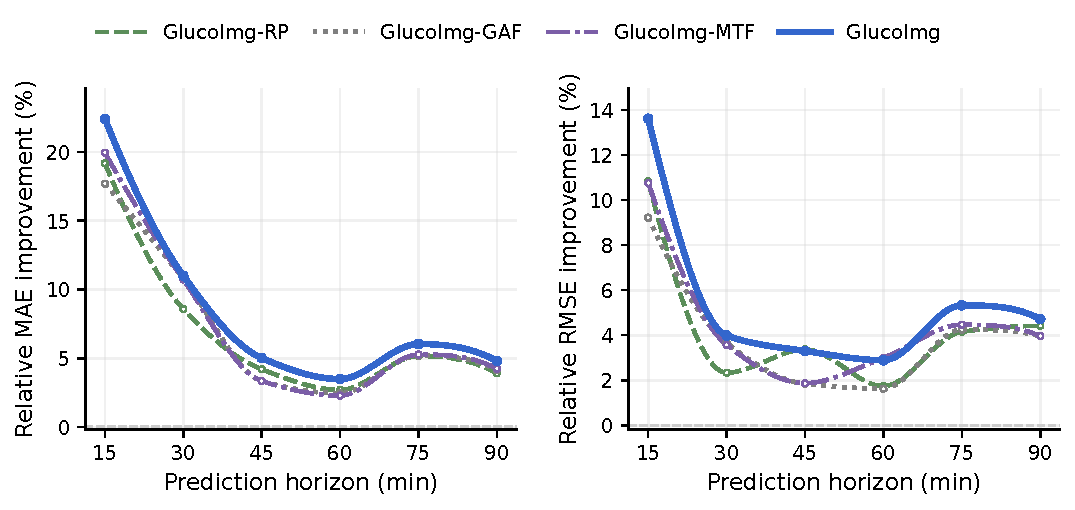
\includegraphics[width=0.92\linewidth]{glucoimg_representation_relative_improvement.pdf}
\caption{Horizon-wise relative forecasting improvement across image representations. Supporting representations are shown as auxiliary comparisons, while GlucoImg denotes the spectrogram-based final model.}
\label{fig:repr_improvement}
\end{figure}

\begin{figure}[t]
\centering
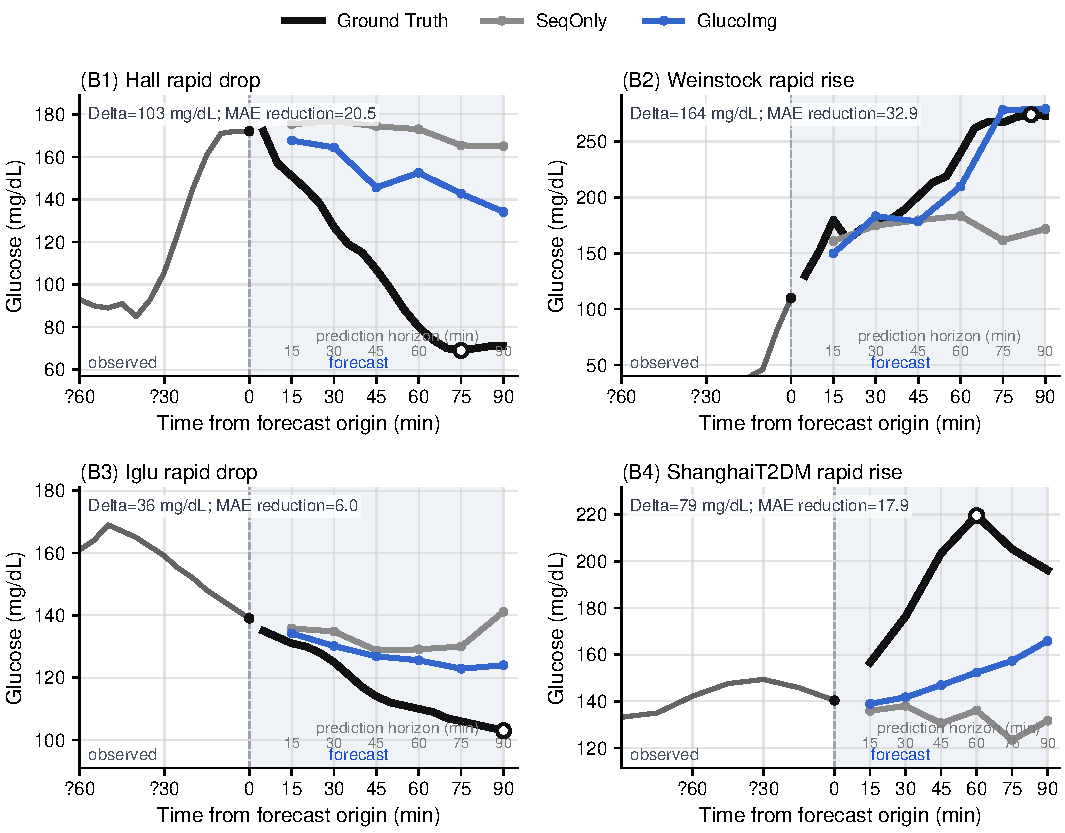
\includegraphics[width=0.95\linewidth]{glucoimg_rapid_transition_cases.pdf}
\caption{Representative rapid-transition cases. GlucoImg more closely follows glucose rise and peak dynamics in selected examples, while SeqOnly tends to lag or smooth rapid changes.}
\label{fig:cases}
\end{figure}

\begin{figure}[t]
\centering
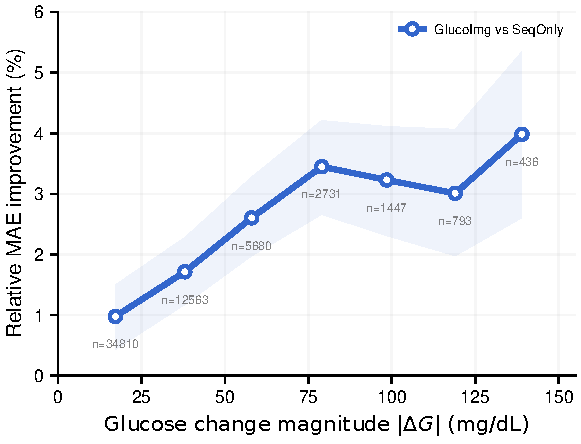
\includegraphics[width=0.8\linewidth]{relative_mae_improvement_vs_glucose_dynamics_rapid_20mgdl_with_n.pdf}
\caption{Relative MAE improvement as a function of true glucose-change magnitude. The increasing trend supports the interpretation that image-enhanced features are more useful when glucose dynamics are stronger.}
\label{fig:dynamics}
\end{figure}

\begin{figure}[t]
\centering
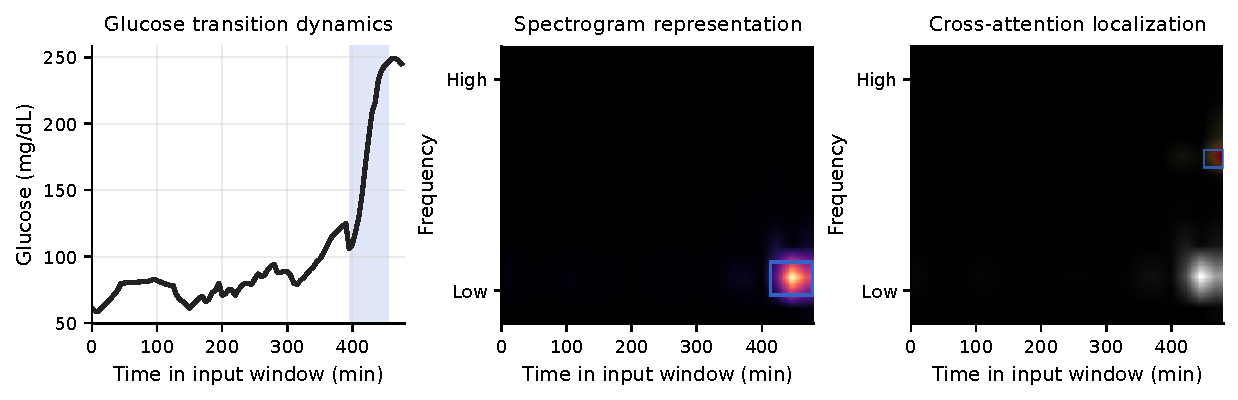
\includegraphics[width=0.95\linewidth]{spectrogram_interpretability_cross_attention.pdf}
\caption{Spectrogram interpretability visualization. A rapid CGM transition corresponds to localized spectrogram energy and patch-level cross-attention activation.}
\label{fig:interpretability}
\end{figure}

\section{Discussion}

This study shows that converting CGM windows into spectrogram images can improve continuous glucose forecasting when the image representation is fused carefully with a strong sequence model. GlucoImg improved average MAE and RMSE over a MambaFormer sequence-only baseline across six prediction horizons. The gains were consistent in the main protocol and remained visible under multiple analyses, including representation ablation, clinical grid evaluation, event detection, and glucose dynamics stratification.

The most important result is not only the average error reduction but the pattern of improvement. GlucoImg was especially helpful for dynamic regimes, including large glucose-change bins and spike-like patterns in the external type 2 diabetes cohort. This supports the hypothesis that spectrogram images expose transition-related structure that is complementary to the raw CGM sequence.

Spectrogram was the best image representation in the main experiment and remained stronger than GAF and MTF in the ShanghaiT2DM trial. A plausible explanation is the alignment between spectrogram structure and patch-token cross-attention. DINOv2 patch tokens preserve local image regions. In spectrograms, local regions can correspond to transient spectral energy associated with rapid glucose changes. Temporal tokens can attend to these local regions through cross-attention. In contrast, RP, GAF, and MTF encode relational or state-transition matrices whose local patches may not correspond as directly to clinically meaningful time-local transitions.

The image branch is not useful for every sample. Stable glucose segments, noisy regions, and some drop patterns may not benefit from spectrogram-derived features. Gated residual fusion addresses this by keeping the sequence-only model as the base forecast and learning an image-driven correction. This design is safer than direct replacement because it allows the model to reduce image influence when the auxiliary representation is not informative.

Clinical utility in glucose forecasting depends on more than average MAE. The Clarke Error Grid results show that GlucoImg improved Zone A predictions most clearly at 90 minutes. Event detection analysis suggests that hyperglycemia detection benefits more consistently than hypoglycemia detection. The ShanghaiT2DM external analysis similarly shows stronger benefit for high-glucose regions and spike patterns than for stable or decreasing glucose states. This pattern supports a clinically specific interpretation: GlucoImg may be more useful for anticipating high-glucose excursions than for uniformly improving every glucose state.

\section{Limitations}

This study has several limitations. First, the image branch uses generated time-series images rather than native medical images. Although this design is intentional, it means that the visual modality is a transformed representation of the same CGM window rather than an independent source of clinical information. Second, DINOv2 was trained on natural images, not CGM-derived spectrograms. Frozen DINOv2 features worked well in the present experiments, but domain-specific self-supervised pretraining on time-series images may further improve performance. Third, ShanghaiT2DM results were horizon-dependent and pattern-specific. GlucoImg did not uniformly outperform SeqOnly in stable or drop patterns, and GAF/MTF did not improve the external validation result. Fourth, event detection for hypoglycemia was less stable than hyperglycemia detection. This may reflect class imbalance, limited hypoglycemia events, and different dynamics for downward glucose transitions. Future work should evaluate additional hypoglycemia-enriched cohorts. Fifth, the current model uses a single image representation in the final architecture. Although All-4 fusion was tested, more sophisticated uncertainty-aware or pattern-aware fusion may be needed to exploit multiple image representations without adding noise.

\section{Conclusion}

We proposed GlucoImg, an image-enhanced glucose forecasting model that combines MambaFormer sequence modeling with spectrogram-derived DINOv2 patch tokens. The model uses cross-attention and gated residual prediction to let visual time-frequency features adaptively correct a sequence-only forecast. Across six horizons, GlucoImg improved average MAE and RMSE over SeqOnly and outperformed alternative image representations and fusion variants. Clinical and dynamics analyses suggest that the benefits are strongest for glucose excursions, particularly high-glucose and spike-like patterns. External ShanghaiT2DM validation showed modest overall gains but clear improvements for 90-minute high-glucose and spike-pattern prediction. These findings support time-series image representations as a useful complement to sequence models for CGM forecasting, while also showing that image enhancement should be interpreted as pattern-specific rather than universally beneficial.

\section*{Data and Code Availability}

The experimental code, processed result tables, and generated figures will be made available upon publication or reasonable request. This statement should be replaced by the final repository link before submission.

\section*{Ethics Statement}

This study uses retrospective CGM datasets from previously published or publicly available cohorts. No prospective intervention was performed. Dataset-specific ethics and consent statements should be verified against the original data sources before submission.

\section*{Acknowledgements}

Acknowledgements should be added after anonymized review, if applicable.

% Uncomment the bibliography block below after replacing the in-text
% [CITATION NEEDED] markers with real \citep{} or \citet{} commands.
% \bibliographystyle{unsrtnat}
% \bibliography{references}

\appendix

\section{Supplementary Notes for Editing}

Before submission, replace all \textbf{[CITATION NEEDED]} markers with verified references. Verify exact dataset names and citations, especially Broll/iGLU, Colas, Dubosson, Hall, Weinstock, and ShanghaiT2DM. Confirm whether the tuned per-horizon table should be reported as the official main result or whether a single unified training run should be used. The 45-minute ShanghaiT2DM SeqOnly MAE in the aggregate table uses the user-provided private rerun value of 13.95; prediction-based clinical analyses still use the original saved prediction files.

\end{document}
